\chapter{Creating an Adventurer}
\label{ch:create-adventurer}
To play in \textbf{Adventure Quest} (\textbf{AQ} for short), you must first create an adventurer to control during the game. All adventurers start out as young persons just leaving home, seeking fame, fortune and yet more adventure. Keep track of your adventurer’s attributes and skills by completing a 4x6 \textbf{adventurer card} like the empty one below; use a pencil for this, as frequent changes will be made during the adventurer’s career.

\begin{tabularx}{\textwidth}{ X l l l l }
\midrule\\
Name: & ( & ) & & Rate\\
STR & Background & & Mod / Defense & Date\\
INT & DP & Combat & / & Silver\\
PER & EU/DU & Missle & / & EXP\\
CSE & Element & Grapple & / & Profession\\
HEA & Languages: & Skills: & Equipment: & Enchanted Items:\\
AGI\\
PWR\\
COM\\
WIL\\[0.25cm]

Race\\
Sex\\
DoB\\
Age\\
Build\\
Height\\
Weight\\
Eye\\
Hair\\
Motive\\
Deity\\
\midrule
\end{tabularx}
\begin{multicols}{2}
\section{Random Numbers}
When people are born, they do not get to choose to be male or female, tall or short, or clever or daft. To simulate this in AQ, these attributes (and other uncontrollable random events) are determined by rolling dice. Later, you may freely choose the skills, languages, etc. your adventurer learns as he grows.\\
Dice come in many different sizes, and when a die roll is required, the type and number are expressed like this:\\
\begin{center}
(\# of dice) d (sides of dice)
\end{center}
Thus, "3d6" means to roll three six-sided dice and add up the results of each die to get the total result. Always assume six-sided dice if the number of sides per die is not specified.
\section{Physical Statistics}
Each adventurer has several attributes. The most important of these are the nine physical statistics or stats, which are listed at the top of the first column of the adventurer card. These stats normally have a rank or value between 0 and 24. These represent:

\begin{tabular}{p{0.2\linewidth} p{0.1\linewidth} p{0.6\linewidth}}
\textbf{Strength} & (STR) & Physical prowess\\
\textbf{Intelligence} & (INT) & Reasoning and problem solving\\
\textbf{Perception} & (PER) & Awareness of surrounding events\\
\textbf{Common Sense} & (CSE) & Sound practical judgement\\
\textbf{Health} & (HEA) & Physical well-being\\
\textbf{Agility} & (AGI) & Physical coordination\\
\textbf{Power} &  (PWR) &  Magical potential\\
\textbf{Comeliness} & (COM) & Physical beauty\\
\textbf{Willpower} & (WIL) & Mental strength\\
\end{tabular}

Each stat is generated by totalling the roll of 3d6, and thus ranges from 3 to 18. Roll 3d6 and write the total op posite STR on the card , roll aga in an d write the total opposite INT, etc. until all stats have a value. Do not despair if they are not all high; playing an adventurer with both strong and weak points is much more fun and interesting than playing an omnipotent adventurer who never needs to think.
\section{Placed Roll}
After rolling the stats, you may change them somewhat to fit the kind of adventurer you wish to play. Roll 4d6 and throw any one die out, totalling the remaining three. Use this total to replace the value of any of your nine original stats. If the roll is unsatisfactory, ignore it and leave your stats unchanged.
\section{Race}
Your adventurer may be one of five different races of intelligent creatures. Members of different races have differing physical appearances and abilities; see \textbf{Chapter \ref{ch:jaern-races}: \nameref{ch:jaern-races}} on page \textbf{\pageref{jh-races}}. Roll 1d20 and check on the following table to determine your adventurer’s race.
\begin{tcolorbox}[breakable,boxrule=0pt]
\begin{tabular}{l l}
Roll & Race\\
\midrule
01 - 14 & Human\\
15 & Elf\\
16 & Dwarf \\
17 & Lizard\\
18 & Orc\\
19 - 20 & Half-breed\\
\end{tabular}
\end{tcolorbox}
If the roll is 19 or 20 this means the adventurer’s parents were of different races. Now roll to find the race of each parent. Each must be a different race, of course, so if the second parent roll is the same as the first, roll again until a different race is determined. The parents may be half-breeds themselves, which means that the adventurer’s grandparents must be determined the same way. If a half-breed grandparent is rolled, ignore it and roll again. Racial heritage determines which racial skills your adventurer has. Non-physical differences are represented as racial skills. For each list below in which your adventurer has a grandparent, roll 1d4 for each skill. If the number is equal to or less than the number of grandparents of that race, write that skill on the adventurer card. If your adventurer is purebred, (i.e., all four grandparents are the same race) he automatically gets all that race's skills. Read the \textbf{Chapter \ref{ch:jaern-humanoids}: \nameref{ch:jaern-humanoids}} to learn about these skills and racial disadvantages.

\begin{multicols}{2}
\textbf{Elf}
\begin{enumerate}
\item Exceptional PER
\item Distance Judgment
\item Missile Skill*
\item Soulless
\end{enumerate}
\textbf{Orc}
\begin{enumerate}
\item Exceptional WIL
\item Enhanced Smell
\item Physical Viciousness*
\item Mental Stubbornness
\end{enumerate}
\textbf{Dwarf}
\begin{enumerate}
\item Exceptional HEA
\item Material Sense
\item Armor Construction*
\item Great Durability
\end{enumerate}
\textbf{Lizard}
\begin{enumerate}
\item Exceptional AGI
\item Quickness
\item Water Breathing
\item Homing
\end{enumerate}
\end{multicols}

*partial breeds check \textbf{Chapter \ref{ch:jaern-races}} to learn how to set these skills.
\nameref{ch:create-adventurer}

Elves are extremely long lived compared to the other races. The do not, however, posses a soul, and thus do not have an existance after death. This makes then unable to use divine magic, and unable to ever be brought back from the dead. Elves generally do not interact with the dieties and their priests. Holy places like temples and shrines make them feel uncomfortable and they tend to avoid them.\\
Full Humans are often more diverse and adaptable than other races. If your adventurer is a full bred human, you may take an additional Placed Roll to further customize your stats. Roll 4d6 and throw any one die out, to talling the remaining three. Use this total to again replace the value of any of your nine original stats. If the roll is unsatisfactory, ignore it and leave your stats unchanged.
\section{Sex}
Choose a sex for your adventurer, or roll 1d6 and
check against the following table:
\begin{tcolorbox}[breakable,boxrule=0pt]
\begin{tabular}{l l}
1 - 3 & Male\\
4 - 6 & Female
\end{tabular}
\end{tcolorbox}
\section{Age}
Determine how old your adventurer is at the start of his or her career by rolling one die of the appropriate type
(from the following table) for each grandparent, and add 10 to the result.
\begin{tcolorbox}[breakable,boxrule=0pt]
\begin{tabular}{l l}
\textbf{Race} & \textbf{Age Die}\\
\midrule
Orc & 4\\
Human & 6\\
Lizards &  8\\
Dwarf & 10\\
Elf &  20\\
\end{tabular}
\end{tcolorbox}
If your adventurer is pure human, obviously all four of his grandparents are human. Roll 4d6, total them and add 10 to find out his age. If, for example, he is half-elf, quarter-human and quarter-dwarf, roll 2d 20 + 1d6 + 1d10 + 10. Aging is covered in detail in \textbf{Chapter \ref{ch:jaern-humanoids}: \nameref{ch:jaern-humanoids}} on page \textbf{\pageref{jh-aging}}.
\section{Body build}
If your adventurer is not purebred, roll 1d4 to randomly select a grandparent’ s race. Now roll 1 d20 to determine your adventurer’s body build using the appropriate race column on the following table. If your adventurer is female, her body build is one catagory smaller than the chart result.
\begin{tcolorbox}[breakable,boxrule=0pt]
\begin{tabular}{l l l l l l}
 & Orc & Elf & Human & Dwarf & Lizard\\
\midrule
A & - & - & - & - & -\\
B & 1 & 1- 2 & - & - & -\\
C & 2- 5 & 3- 6 & 1- 2 & - & -\\
D & 6-16 & 7-14 & 3- 6 & 1 & 1- 2\\
E & 17-19 & 15-18 & 7-14 & 2- 5 & 3- 6\\
F & 20 & 19-20 & 15-18 & 6-16 & 7-14\\
G & - & - & 19-20 & 17-19 & 15-18\\
H & - & - & - & 20 & 19-20\\
\end{tabular}
\end{tcolorbox}
\end{multicols}
\section{Height and Weight}
Height and weight are determined by rolling 4d6 and totalling them. Add the number shown below for the race of each grandparent.
\begin{tcolorbox}[breakable,boxrule=0pt]
\begin{tabular}{l l}
Dwarves & +0\\
Orcs & +2\\
Humans & +4\\
Elves & +5\\
Lizards & +6\\
\end{tabular}
\end{tcolorbox}
\begin{center}
\large
Height and Weight Table\\
\end{center}
\normalsize
\begin{tcolorbox}[breakable,boxrule=0pt]
\begin{tabular}{l l l l l l l l l l}
ROLL & height & A & B & C & D & E & F & G & H\\
\midrule
4 & 3'7" & 29 & 35 & 42 & 51 & 62 & 74 & 89 & 108\\
5 & 3'8" & 31 & 37 & 44 & 54 & 65 & 78 & 94 & 113\\
6 & 3'9" & 32 & 39 & 47 & 56 & 68 & 81 & 98 & 118\\
7 & 3'10" & 34 & 40 & 49 & 59 & 71 & 85 & 103 & 124\\
8 & 3'11" & 35 & 42 & 51 & 61 & 74 & 89 & 107 & 129\\
9 & 4'0" & 37 & 44 & 53 & 64 & 77 & 93 & 112 & 135\\
10 & 4'1" & 38 & 46 & 55 & 67 & 80 & 97 & 117 & 141\\
11 & 4'2" & 40 & 48 & 58 & 70 & 84 & 101 & 122 & 146\\
12 & 4'3" & 41 & 50 & 60 & 72 & 87 & 105 & 127 & 153\\
13 & 4'4" & 43 & 52 & 63 & 75 & 91 & 109 & 132 & 159\\
14 & 4'5" & 45 & 54 & 65 & 78 & 94 & 114 & 137 & 165\\
15 & 4'6" & 47 & 56 & 68 & 81 & 98 & 118 & 142 & 171\\
16 & 4'7" & 48 & 58 & 70 & 85 & 102 & 123 & 148 & 178\\
17 & 4'8" & 50 & 60 & 73 & 88 & 106 & 127 & 153 & 185\\
18 & 4'9" & 52 & 63 & 75 & 91 & 110 & 132 & 159 & 192\\
19 & 4'10" & 54 & 65 & 78 & 94 & 114 & 137 & 165 & 199\\
20 & 4'11" & 56 & 67 & 81 & 98 & 118 & 142 & 171 & 206\\
21 & 5'0" & 58 & 70 & 84 & 101 & 122 & 147 & 177 & 213\\
22 & 5'1" & 60 & 72 & 87 & 105 & 126 & 152 & 183 & 220\\
23 & 5'2" & 62 & 75 & 90 & 108 & 130 & 157 & 189 & 228\\
24 & 5'3" & 64 & 77 & 93 & 112 & 135 & 162 & 196 & 236\\
25 & 5'4" & 66 & 80 & 96 & 116 & 139 & 168 & 202 & 243\\
26 & 5'5" & 68 & 82 & 99 & 119 & 144 & 173 & 209 & 251\\
27 & 5'6" & 70 & 85 & 102 & 123 & 148 & 179 & 215 & 259\\
28 & 5'7" & 73 & 88 & 105 & 127 & 153 & 184 & 222 & 268\\
29 & 5'8" & 75 & 90 & 109 & 131 & 158 & 190 & 229 & 276\\
30 & 5'9" & 77 & 93 & 112 & 135 & 163 & 196 & 236 & 285\\
31 & 5'10" & 80 & 96 & 115 & 139 & 168 & 202 & 243 & 293\\
32 & 5'11" & 82 & 99 & 119 & 143 & 173 & 208 & 251 & 302\\
33 & 6'0" & 84 & 102 & 122 & 148 & 178 & 214 & 258 & 311\\
34 & 6'1" & 87 & 105 & 126 & 152 & 183 & 220 & 266 & 320\\
35 & 6'2" & 89 & 108 & 130 & 156 & 188 & 227 & 273 & 329\\
36 & 6'3" & 92 & 111 & 133 & 161 & 194 & 233 & 281 & 339\\
37 & 6'4" & 94 & 114 & 137 & 165 & 199 & 240 & 289 & 348\\
38 & 6'5" & 97 & 117 & 141 & 170 & 205 & 246 & 297 & 358\\
39 & 6'6" & 100 & 120 & 145 & 174 & 210 & 253 & 305 & 368\\
40 & 6'7" & 102 & 123 & 149 & 179 & 216 & 260 & 313 & 377\\
41 & 6'8" & 105 & 127 & 153 & 184 & 222 & 267 & 322 & 388\\
42 & 6'9" & 108 & 130 & 157 & 189 & 227 & 274 & 330 & 398\\
43 & 6'10" & 111 & 133 & 161 & 194 & 233 & 281 & 339 & 408\\
44 & 6'11" & 114 & 137 & 165 & 199 & 239 & 288 & 348 & 419\\
45 & 7'0" & 117 & 140 & 169 & 204 & 246 & 296 & 356 & 429\\
46 & 7'1" & 119 & 144 & 173 & 209 & 252 & 303 & 365 & 440\\
47 & 7'2" & 122 & 148 & 178 & 214 & 258 & 311 & 374 & 451\\
48 & 7'3" & 125 & 151 & 182 & 219 & 264 & 318 & 384 & 462\\
\end{tabular}
\end{tcolorbox}
\pagebreak
\begin{multicols}{2}
\normalsize
\section{Eye color}
If your adventurer is not purebred, roll 1d4 to randomly select a grandparent's race. Now roll 1d20 to find your adventurer's eye color, using the apropriate race column on this table:

\begin{tcolorbox}[breakable,boxrule=0pt]
\begin{tabular}{l l l l l l}
Color & Human & Elf & Dwarf & Orc & Lizard\\
\midrule
Black & 1 & 1-2 & 1-10 & 1-4 & 1-12\\
Brown & 2-8 & -- & 11-18 & 5-6 & --\\
Blue & 9-14 & 3-10 & -- & -- & 13-15\\
Green & 15-16 & 11-14 & 19-20 & 7-12 & 16\\
Red & -- & 15-17 & -- & 13-18 & 17-19\\
Silver & -- & 18-19 & -- & -- & 20\\
Hazel & 17-20 & -- & -- & 19-20 & --\\
White & -- & 20 & -- & -- & --
\end{tabular}
\end{tcolorbox}

\section{Hair color}
If your adventurer is not purebred, roll 1d4 to randomly select a grandparent's race. Now roll 1d20 to find your adventurer's hair color, using the apropriate race column on this table:
\begin{tcolorbox}[breakable,boxrule=0pt]
\begin{tabular}{l l l l l l}
Color & Human & Elf & Dwarf & Orc & Lizard\\
\midrule

Brown & 1-7 & -- & 1-10 & 1-2 & --\\
Black & 8-11 & 1-6 & 11-16 & 3-16 & --\\
Blond & 12-15 & 7-8 & -- & -- & --\\
Red & 16-17 & 9-13 & 17 & 17-18 & --\\
Green & -- & 14-15 & -- & 19 & --\\
Grey & 18 & -- & 18 & -- & --\\
White & 19 & 16-18 & -- & 20 & --\\
None & 20 & -- & 19-20 & -- & 1-20\\
Silver & -- & 19-20 & -- & -- & --
\end{tabular}
\end{tcolorbox}
\section{Motivation}
That takes care of the random elements of adventurer creation; now you have a free hand in developing your adventurer’s inner-self. Evolving his personality takes some thought, but it is a rewarding aspect of roleplaying. A good way to start is to create an event that occurred early in his life that now defines his basic motivation. Once you have a starting point it is easier to describe more about their personality.
Below are some possible motivations from which to choose, but you are free to make up others as best fits your needs and concepts. Now mentally describe an event or condition to explain why it is your adventurer's primary motivation. Write this motive down on the Adventurer Card after "Motive." Here are some suggestions:

\begin{tabular}{l l}
Duty & Alliegance to a higher authority\\
Fame & Gaining recognition from others\\
Justice & Maintaining balance\\
Knowledge & Learning for learning’s sake\\
Passion & Serving a cause with intense emotional fervor\\
Pleasure & Seeking pleasures of the flesh\\
Power & Forcing the submission of others\\
Religion & Devoting their life to a higher authority\\
Righteousness & Striving to helpmankind\\
Romance & Earning the love and/or respect of others
\end{tabular}

The motive you choose is not meant to be a "straight jacket" to force you to play the adventurer within narrow bounds. It is meant to be used, by you, to help set a direction for your adventurer’s actions and a start for his personality. You always have the freedom to write down what you believe is your adventurer’s driving force on your card. Also realize that there is magic which can be used to determine your motive, and the results of this magic will be what is percieved by the GM as your motive, which may disagree with what you have written.
To learn more about creating your adventurer's personality, read \textbf{Chapter \ref{ch:creating-actors}: \nameref{ch:creating-actors}} to see how the GM creates personalities for actors. These methods are applicable to your adventurer’s personality as well.
\section{Patron Gods}
You may select one deity as your adventurer’s patron god. Adventurers aligning themselves to a deity this way are expected to assist the causes of the god, and especially to follow that god’s precepts and laws. In return, they are often assisted by the priests and followers of that deity. Worshipping more than one god is possible, but can become difficult if the deities conflict in any way. Write down the name(s) of the deity(s) on the adventurer card after "Deity." Here is a list of available deities; each is covered in detail in its own chapter.

\begin{tabular}{l l l}
\textbf{GOD} & \textbf{Sphere of Influence} & \textbf{Sex}\\
Ra & Bearer of Light & M\\
Isis & Mistress of Life & F\\
T’or & The Thunder of Righteousness & M\\
At’ena & Mistress of Wisdom & F\\
Osiris & Protector of Nature & F\\
Tarus & Master Archivist & M\\
Neptune & Dweller of the Waters & M\\
Orus & The Flame of Zeal & M\\
Anubis & Lord of the Dead & M\\
Rudri & Dweller of the Dark & F\\
Scrogg & Concubine and follower of Orus & M\\
\end{tabular}
\section{Adventurer Background}
Backrounds are the adventuring professions available in a specific AQ Game. Each Game has at least three major, divergent disciplines that may be followed, and thus gives three professions. Others are derived by combining two of the major disciplines to yield another, unique background.\\
It may be helpful for you to visualize this as a three-spoked wheel, each spok labeled witha a major discipline. In AQ/Jaern these are Combat, Magic, and Skills.

\begin{center}

\tikzset{every picture/.style={line width=0.75pt}} %set default line width to 0.75pt        

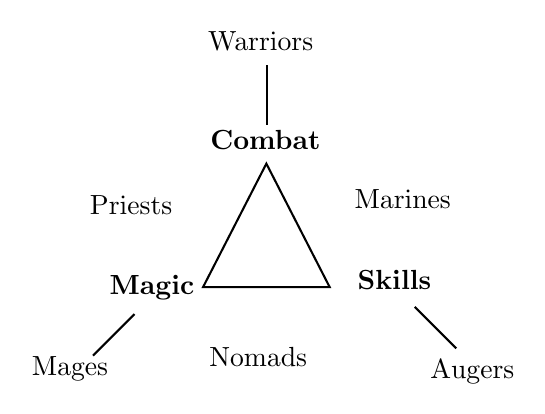
\begin{tikzpicture}[x=0.75pt,y=0.75pt,yscale=-1,xscale=1]
%uncomment if require: \path (0,300); %set diagram left start at 0, and has height of 300

%Straight Lines [id:da5792073549069615] 
\draw    (321.5,53) -- (321.5,82) ;
%Shape: Triangle [id:dp9921269194788708] 
\draw   (321,100.5) -- (351.5,160) -- (290.5,160) -- cycle ;
%Straight Lines [id:da10414083526965556] 
\draw    (257.5,173) -- (237.5,193) ;
%Straight Lines [id:da8045071749370871] 
\draw    (392.5,169.5) -- (412.5,189.5) ;

% Text Node
\draw (291.5,35.5) node [anchor=north west][inner sep=0.75pt]   [align=left] {Warriors};
% Text Node
\draw (234.5,114.5) node [anchor=north west][inner sep=0.75pt]   [align=left] {Priests};
% Text Node
\draw (362,111.5) node [anchor=north west][inner sep=0.75pt]   [align=left] {Marines};
% Text Node
\draw (206.5,192) node [anchor=north west][inner sep=0.75pt]   [align=left] {Mages};
% Text Node
\draw (292,187.5) node [anchor=north west][inner sep=0.75pt]   [align=left] {Nomads};
% Text Node
\draw (398.5,193.5) node [anchor=north west][inner sep=0.75pt]   [align=left] {Augers};
% Text Node
\draw (363.5,150.5) node [anchor=north west][inner sep=0.75pt]   [align=left] {\textbf{Skills}};
% Text Node
\draw (244,153) node [anchor=north west][inner sep=0.75pt]   [align=left] {\textbf{Magic}};
% Text Node
\draw (292.5,83) node [anchor=north west][inner sep=0.75pt]   [align=left] {\textbf{Combat}};


\end{tikzpicture}
\end{center}

The three backgrounds at the ends of the spokes are thus Warrior (for those exclusively trained in combat) Mages (Magic), and Augers (Skills). As for the areas between the spokes, a background that combines Magic and Combat produces the Priest, someone with a knowledge of Magic and the physical training to back it up. Combining Magic and skills yields a Nomad, with training in the mystical arts as well as skills. And finally, mixing Combat and Skills produces a Marine, a person with a need for fighting ability and quick and nimble movements.

\begin{tabular}{l l}
\textbf{Adventurer Background} & \textbf{Most Important Stat}\\
\midrule
Warrior & CSE and STR\\
Priest &  PWR and CSE\\
Magician &  PWR and INT\\
Nomad &  PER and HEA\\
Auger &  INT and CSE\\
Marine &  AGI and STR
\end{tabular}

Each background has one or more stats that is very important to the successful practice of the profession, as given in the above table. If your adventurer’s highest stat is
STR, they probably would fare best as a Warrior. If they have a high PER, you probably should consider making them a Nomad, etc.\\
You must now choose an available background for your adventurer. Consider not only the stats, but also what you envision your persona becoming, or what you want to roleplay. You are not forced to pick the background that matches the highest stat. In fact, successfully roleplaying (for example) an adventurer with a high STR and a mediocre INT as a Auger rather than a Warrior is very rewarding, not to mention entertaining, to you, the GM, and other players.Here are descriptions of the available backgrounds to further help you make a selection:\\
\begin{itemize}
\item A \textbf{Warrior} relies upon their skill at arms. They are proficient at fighting and confident in their ability to succeed with force. While they might serve in an army, a warrior prefers individual combat and is more likely found employed as a bodyguard, mercenary, constable, or a guard.
\item A \textbf{Priest} is devoted to the service of a deity, forever at that deity's disposal to spread their faith and worship throughout the world. A priest is willing for fight for their deity’s cause, but can also use god-given magical powers to further their goals.
\item A \textbf{Magician} is a practitioner of one of four types of elemental magics, using his magics to affect the world and gain wealth, recognition and influence. A magician is often consulted and employed by others to accomplish their goals.
\item The spells available in each element give a definite flavor to the personality and style of play of a magician. Fire and Air magicians tend to have more offensive spells, whereas Earth and Water mages are more defense oriented. Fire and Earth magic tends to be more individual in nature, while many Air and Water spells are useful to support and maintain a group of adventurers. If your adventurer is going to become a magician, bear these generalities in mind to select the elemental style that matches your adventurer's personality.
\item Brought up learning to think to solve their problems, an Auger’s basic tenet is to live up to their potential, learning to utilize their best skills and making the most of any situation.
\item Born to the seas, a \textbf{Marine} is a member of the traveling armies that plies the seas of Jaern. Ready with a quick story of marine heroes of the past, today's marine attempts to make a name for themseves and their shipmates. They adventure for fame, and are always ready for a good fight and a large tankard of ale.
\item Members of a tight-knit group of families, \textbf{Nomads} mistrust all other Jaernians and rarely travel among them. They are rumored to have various mystical and magical powers, so most people shun them, unsure of their intentions.
\end{itemize}
After choosing one of these, place it on the adventurer card after "Background." If you’re still uncertain, scan the list of Model Adventurers beginning on page \textbf{\pageref{adventurer-models}} for ideas and suggestions.\\
If it appears your adventurer suffers from hopelessly inadequate stats, they would probably not become an adventurer in a fantasy world. Ask the GM; they may allow you to discard this would-be adventurer and start over.
\section{Languages}
You need to know which languages (if any) your adventurer speaks to know how they can communicate with actors and other adventurers. Knowledge of languages is an intelligence-based skill, and beginning adventurers may know zero, one or two languages.
\begin{tcolorbox}[breakable,boxrule=0pt]
\begin{tabular}{l l l}
INT & Initial Languages & Maximum Languages\\
\midrule
3 - 5 & 0 & 0\\
6 - 8 & 1 & 1\\
9 - 11 & 2 & 2\\
12 - 14 & 2 & 3\\
15 - 17 & 2 & 4\\
18 - 20 & 2 & 5\\
21 - 23 & 2 & 6\\
24+ & 2 & 7\\
\end{tabular}
\end{tcolorbox}
Adventurers having an INT of less than 6 cannot speak coherently. They may know how to say isolated wordsor phrases, and can generally understand simple sentences. Playing adventurers with a low INT is very challenging because the player must communicate through actions rather than words. \\
The first language an adventurer with an INT greater than 6 learns is his racial language. This is Paroli for all human adventurers. Half-breed adventurers may pick one of their racial languages as their native tongue or the tongue of whomever raised him, whichever is most appropriate. The first language is always known at a skill rank of 9 or the adventurer’s INT, whichever is lower.\\
With an INT above 8, the player may choose a second language. For non-human adventurers, it would be prudent to pick the common tongue of the area to simplify communications. This second language is initially known at a skill rank of 6.

The available languages are:

\begin{tabular}{p{0.2\linewidth} p{0.7\linewidth}}
Breziak & human tongue\\
Dwarvish & race tongue of dwarves\\
Elvish & race tongue of most elves\\
Entish & spoken by intelligent forest creatures\\
Ferric & human tongue\\
Geleik & tongue of the elves of Silvan Isle\\
Haoogh & speech of the southern pirates\\
Orcish & race tongue of orcs\\
Paroli & race tongue for humans and common tongue\\
Sel’ict & race tongue of the lizard men\\
Trejon & ancient human tongue\\
\end{tabular}
\section{Rating}
Your GM must be able to balance your adventuring party against some opponents it might meet. Your adventurer's \textbf{Rating} is how many adventurers they have experienced. Set this at two now, and each time he finishes a gaming session, add one. A starting rating of two represents the skills that you choose in creating your adventurer. Your GM may ask for this number from all the players at the beginning of a gaming session.
\section{Date}
At the beginning and end of each adventure, the Game Master will tell you the current game date. The amount of time elapsed between adventures is important for curing damage, doing research, being pregnant, etc. The date is in ISO 8601 format (Year-Month-Day), such as 10080-06-15 SF (Since Founding). Record the current date minus your age on your card as your date of birth (DOB).
\section{Nomadic Prefix Names}
If your adventurer is a nomad, then they must know their own prefix name, or \textbf{epokonom}. Roll 1d20 and look at this table:
\begin{tcolorbox}[breakable,boxrule=0pt]
\begin{tabular}{l l|l l}
Roll & Epokonom & Roll & Epokonom\\
\midrule
1 - 5 & Raz- & 16 & Ald-\\
6 - 9 & Car- & 17 & Edo-\\
10 - 12 & Oka- & 18 & Ijo-\\
13 - 14 & Vem- & 19 & Bez-\\
15 & Lar- & 20 & Sag-\\
\end{tabular}
\end{tcolorbox}
Put this prefix before your adventurer’s name.
\section{Name}
Each adventurer must have a name of some sort. Choose a name for your adventurer and place it in the upper left-hand corner of the card. After this put your real name in parenthesis. This will help the Game Master to remember whose adventurer is whose.
\section{Profession}
Your adventurer may have a regular job to bring in a steady income. After your adventurer’s skills are selected (see page \textbf{\pageref{create-skills}}), you may choose one as their profession.
\section{Adventurer Models}
Players buy attributes for their adventurers using experience points. Physical equipment is bought with silver pieces. This buying allows you to make your adventurer’s abilities fit your perception of her personality.\\
To simplify making a new adventurer, several different Model Adventurers are reproduced here. If you wish to pick one of these, just copy the information from the chosen model that matches your adventurer’s background onto an adventurer card. For each defense value listed in the model, plug in the appropriate stats from your adventurer (dividing them by 5 and rounding down as shown) and add the results to find the your adventurer’s defense values. If they are an elf, add one on their MDV for Exceptional PER. If they are an orc, add one to his GDV for Exceptional WIL. Your adventurer is ready to play.\\
Each model allows you 20\% more attributes than if you had bought all the attributes separately. This extra does not make the adventurer more powerful; it is used to buy attributes that give added flavor and a direction for further development. Once selected, models cannot be modified or changed except to buy new attributes (or upgrade current ones) with earned experience points (see \nameref{create-buying} on page \textbf{\pageref{create-buying}}).
If none of the models fit your idea of your adventurer’s personality, and your GM is allowing custom a dventurer creation, skip this section and read \nameref{create-buying} to learn how to complete your adventurer’s creation.\\
Each adventurer prototype specifies the values for the following attributes:
\end{multicols}
\begin{tabular}{l l}
Damage Points (DP) & Relative health\\
Combat Modifier (CM) & Ability using hand-to-hand weapons\\
Missile Modifier (MM) & Ability using bows, slings and crossbows\\
Grapple Modifier (GM) & Ability to grapple\\
Spell type & Declared type of spells (EARTH, FIRE, AIR, WATER, and DIVINE)\\
Spell Groups & Ability to use various spell groups\\
Incants & Specific nomadic items and tailsmen\\
Skills & Purchased skills and their ranks\\
Combat Defense (CDV) & Resistance to being struck\\
Missile Defense (MDV) & Resistance to being hit by missiles\\
Grapple Defense (GDV) & Resistance to being grappled\\
\end{tabular}
\begin{multicols}{2}
\subsection{Models}
TBD
\section{Experience Points}
Experience Points (EP) are the currency used to buy such attributes as skills, stats, spells groups, damage points, and melee modifiers. Your adventurer is awarded EP during and after an adventure in several ways, depending on the method chosen by your GM. Using experience points in this way simulates any training or study that might be required to acquire or improve an ability without actually going through the tedium and boredom of doing so during a gaming session. By the way, when an adventure ends, don’t forget to add one to the Rating entry on the adventurer’s card. Your GM uses the Rating to get a rough idea of how much experience your adventurer has had so that they may balance the difficulty of an adventure against the power of the adventurers.\\
You may specify that a portion of the awarded experience be set aside and used later to buy attributes. There is no limit to the amount of experience your adventurer may hold, but it makes little sense to hold it longer than needed to buy the attributes sought.
\section{Buying}
\label{create-buying}
If you have not chosen an Adventurer Model, your adventurer is given 5,000 EP with which to buy:

\begin{tabular}{l l}
STATS & such as STR, INT, etc.\\
DAMAGE POINTS  & the ability to survive injury\\
MELEE MODs & abiltiy to resist physical damage\\
SPELLS & magician and priest magic\\
INCANTS & nomadic rituals\\
LANGUAGES & spoken languages\\
ABILITIES & useful skills and abilities\\
\end{tabular}

All buying must be done either when creating an adventurer or between adventures, and must be witnessed by the GM or their representative. The majority of the time this will be done when the adventurer has returned to a civilized setting, where the resources for training are most likely to be found. If an adventure is one in a series, and no game time has passed since the previous adventure, your GM may disallow buying attributes until after the entire sequence of adventures has been completed. \\
All attributes start at an initial rank of zero and may be bought upward one point at a time. To buy new attributes, or increase the value of an old one, multiply the base cost of the attribute by the point value you wish your adventurer to gain.

\textit{If Marna (a priestess of Osiris) attempts to raise her teaching skill (base cost 100 EP) from 8 to 9, she must expend 100 x 9 or 900 EP to do so.\\
If George the Magnificient (a Warrior) wants to raise his disguise attribute (base cost 50 EP) from 11 to 12, it will cost him 12 x 50 x 3 or 1800 EP. The 3x multiplier is included because the skill is an Auger skill, and George is a Warrior. See \nameref{create-skills} on page \textbf{\pageref{create-skills}} for more information on purchasing skills outside your class.}
\subsection{Buying up from zero}
While attributes are usually bought one point at a time, sometimes it is necessary to buy one from zero up to a high value. To do this, we use a little bit of math . . .\\
To buy something from zero to an arbitrary value, call that value N,

$Total Cost = \frac{N * (N+1)}{2} * Base Cost$

For example, to buy damage points (base cost 25 EP) from zero up to 16 would cost as follows:

$\frac{16 * (16+1)}{2} * 25 = \frac{16*17}{2} * 25 = 3,400 EP$

If the formula above is too intimidating, use the following table. Cross reference your adventurer’s current rank in the attribute against the desired rank, then multiply the number from the table by the base cost of the attribute to find the experience point cost.

\end{multicols}
\begin{tcolorbox}[breakable,boxrule=0pt]
\begin{tabular}{l l l l l l l l l l l l l l l l l l l}
\textbf{OLD} & \multicolumn{16}{c}{\textbf{NEW RANK}}\\
\textbf{RANK} & \textbf{1} & \textbf{2} & \textbf{3} & \textbf{4} & \textbf{5} & \textbf{6} & \textbf{7} & \textbf{8} & \textbf{9} & \textbf{10} & \textbf{11} & \textbf{12} & \textbf{13} & \textbf{14} & \textbf{15} & \textbf{16} & \textbf{17} & \textbf{18}\\
0 & 1 & 3 & 6 & 10 & 15 & 21 & 28 & 36 & 45 & 55 & 66 & 78 & 91 & 105 & 120 & 136 & 153 & 171\\
1 & -- & 2 & 5 & 9 & 14 & 20 & 27 & 35 & 44 & 54 & 65 & 77 & 90 & 104 & 119 & 135 & 152 & 170\\
2 & -- & -- & 3 & 7 & 12 & 18 & 25 & 33 & 42 & 52 & 63 & 75 & 88 & 102 & 117 & 133 & 150 & 168\\
3 & -- & -- & -- & 4 & 9 & 15 & 22 & 30 & 39 & 49 & 60 & 72 & 85 & 99 & 114 & 130 & 147 & 165\\
4 & -- & -- & -- & -- & 5 & 11 & 18 & 26 & 35 & 45 & 56 & 68 & 81 & 95 & 110 & 126 & 143 & 161\\
5 & -- & -- & -- & -- & -- & 6 & 13 & 21 & 30 & 40 & 51 & 63 & 76 & 90 & 105 & 121 & 138 & 156\\
6 & -- & -- & -- & -- & -- & -- & 7 & 15 & 24 & 34 & 45 & 57 & 70 & 84 & 99 & 115 & 132 & 150\\
7 & -- & -- & -- & -- & -- & -- & -- & 8 & 17 & 27 & 38 & 50 & 63 & 77 & 92 & 108 & 125 & 143\\
8 & -- & -- & -- & -- & -- & -- & -- & -- & 9 & 19 & 30 & 42 & 55 & 69 & 84 & 100 & 117 & 135\\
9 & -- & -- & -- & -- & -- & -- & -- & -- & -- & 10 & 21 & 33 & 46 & 60 & 75 & 91 & 108 & 126\\
10 & -- & -- & -- & -- & -- & -- & -- & -- & -- & -- & 11 & 23 & 36 & 50 & 65 & 81 & 98 & 116\\
11 & -- & -- & -- & -- & -- & -- & -- & -- & -- & -- & -- & 12 & 25 & 39 & 54 & 70 & 87 & 105\\
12 & -- & -- & -- & -- & -- & -- & -- & -- & -- & -- & -- & -- & 13 & 27 & 42 & 58 & 75 & 93\\
13 & -- & -- & -- & -- & -- & -- & -- & -- & -- & -- & -- & -- & -- & 14 & 29 & 45 & 62 & 80\\
14 & -- & -- & -- & -- & -- & -- & -- & -- & -- & -- & -- & -- & -- & -- & 15 & 31 & 48 & 66\\
15 & -- & -- & -- & -- & -- & -- & -- & -- & -- & -- & -- & -- & -- & -- & -- & 16 & 33 & 51\\
16 & -- & -- & -- & -- & -- & -- & -- & -- & -- & -- & -- & -- & -- & -- & -- & -- & 17 & 35\\
\end{tabular}
\end{tcolorbox}
\begin{multicols}{2}
\section{Stats}
Of all the attributes, stats are arguably the most important. Stats are the basis for most resistance checks (the avoidance of effects), and determine the maximum value for most other attributes (skills, languages, spell groups, etc.). At a base cost of 500, they are also very expensive to increase. For example, to buy STR from 14 to 15 would cost 500 x 15 = 7,500 experience points.
\hrule
\textit{Optional:\\
A physical stat may not be increased more than 4 above the initial roll, to reflect the notion that training and practice can only increase a physical ability so much.}
\hrule
\section{Damage Points}
Damage points (DP) indicate your adventurer's ability to avoid damage during combat. As you buy this total higher, your adventurer becomes more skillful at dodging, moving and twisting to avoid being damaged while fighting. If they are injured, damage points are temporarily subtracted from their totral DP; the new total indicates their relative condition.
Lost DP may be regained by resting. A full night’s rest (at least eight hours; twelve for those with no soul, like elves) restores a number of DP equal to the adventurer’s HEA divided by five (by two for those with the Exceptional HEA skill, like most dwarves), rounded down. Damage points may not be restored beyond the original maximum DP total. \\
The base cost for DPs is 25. Your adventurer must have DPs to survive, so here is a chart of the total cost of buying damage points up from zero.

\begin{tcolorbox}[breakable,boxrule=0pt]
\begin{tabular}{l l|l l|l l}
DP & Cost & DP & Cost & DP & Cost\\
\midrule
1 & 25 & 8 & 900 & 15 & 3000\\
2 & 75 & 9 & 1125 & 16 & 3400\\
3 & 150 & 10 & 1375 & 17 & 3825\\
4 & 250 & 11 & 1650 & 18 & 4275\\
5 & 375 & 12 & 1950 & 19 & 4750\\
6 & 525 & 13 & 2275 & 20 & 5250\\
7 & 700 & 14 & 2625 & 21 & 5775\\
\end{tabular}
\end{tcolorbox}

Buying damage points with experience actually simulates additional training to avoid being wounded. This could be handled as another defensive modification, but being able to take more damage yields the same effect, is easier to keep track of, balances quite nicely, and is more fun to play.\\
When buying damage points, you are only increasing your adventurer’s maximum DP, not their current DP total. New DPs are only gained after resting, according to the DP recovery rule above.
\section{Melee Modifiers}
Every adventurer has three modifiers, or Mods, that help determine success in combat. The \textbf{Combat Modifier (CM)} is added to all 1d20 "to strike" rolls you make when
your adventurer attacks using a hand-to-hand weapon. The \textbf{Missile Modifier (MM)} is added to all "to hit" rolls from bows, crossbows and thrown objects. The \textbf{Grapple Modifier (GM)} is used when wrestling or boxing an opponent. Mods start at rank zero and are bought upward like any other attribure. The base cost depends on your adventurer’s background:

\begin{tcolorbox}[breakable,boxrule=0pt]
\begin{tabular}{l l l l}
\textbf{Background} & \textbf{Combat} & \textbf{Missile} & \textbf{Grapple}\\
\midrule
Warrior & 200 & 200 & 200\\
Priest & 300 & 300 & 400\\
Mage & 400 & 500 & 600\\
Nomad & 500 & 600 & 500\\
Auger & 400 & 400 & 400\\
Marine & 300 & 400 & 200\\
\end{tabular}
\end{tcolorbox}
Subtract the calculated \textbf{EP} from your adventurer’s expendable EP total, then place the values for these on the \textbf{Adventurer Card} after \textbf{Combat}, \textbf{Missile}, and \textbf{Grapple}.
\section{Spells}
\subsection{Acquiring Spells from Other Elements}
\subsection{Stat Limitations}
\subsection{Buying of Spells by Other Backgrounds}
\section{Incants}
\subsection{Preparing of Incants by Other Backgrounds}
\section{Languages}
\section{Skills}
\label{create-skills}
\subsection{Larning Skills}
\section{Money}
\section{Equipment}
\section{Defense Values}
\subsection{Mobility}
\subsection{Agility}
\subsection{Stat Modifiers}
\subsection{Armor}
\subsection{Defensive Devices}
\subsection{Weapons}
\end{multicols}